% \iffalse
\let\negmedspace\undefined
\let\negthickspace\undefined
\documentclass[journal,12pt,twocolumn]{IEEEtran}
\usepackage{cite}
\usepackage{amsmath,amssymb,amsfonts,amsthm}
\usepackage{algorithmic}
\usepackage{graphicx}
\usepackage{textcomp}
\usepackage{xcolor}
\usepackage{txfonts}
\usepackage{listings}
\usepackage{enumitem}
\usepackage{mathtools}
\usepackage{gensymb}
\usepackage{comment}
\usepackage[breaklinks=true]{hyperref}
\usepackage{tkz-euclide} 
\usepackage{listings}
\usepackage{gvv}                                        
\def\inputGnumericTable{}                                 
\usepackage[latin1]{inputenc}                                
\usepackage{color}                                            
\usepackage{array}                                            
\usepackage{longtable}                                       
\usepackage{calc}                                             
\usepackage{multirow}                                         
\usepackage{hhline}                                           
\usepackage{ifthen}                                           
\usepackage{lscape}
\usepackage[center]{caption} % center the captions to figure

\newtheorem{theorem}{Theorem}[section]
\newtheorem{problem}{Problem}
\newtheorem{proposition}{Proposition}[section]
\newtheorem{lemma}{Lemma}[section]
\newtheorem{corollary}[theorem]{Corollary}
\newtheorem{example}{Example}[section]
\newtheorem{definition}[problem]{Definition}
\newcommand{\BEQA}{\begin{eqnarray}}
\newcommand{\EEQA}{\end{eqnarray}}
\newcommand{\define}{\stackrel{\triangle}{=}}
\theoremstyle{remark}
\newtheorem{rem}{Remark}
\begin{document}

\newcolumntype{M}[1]{>{\centering\arraybackslash}m{#1}}
\newcolumntype{N}{@{}m{0pt}@{}}

\bibliographystyle{IEEEtran}
\vspace{3cm}

\title{NCERT Physics 12.10.9 Q} 
\author{ee23btech11223 - Soham Prabhakar More% <-this % stops a space
}
\maketitle
\newpage
\bigskip

\renewcommand{\thefigure}{\theenumi}
\renewcommand{\thetable}{\theenumi}

\bibliographystyle{IEEEtran}

\textbf{Question:} Light of wavelength $5000\AA{}$ falls on a plane reflecting surface. What
are the wavelength and frequency of the reflected light? For what
angle of incidence is the reflected ray normal to the incident ray?\\

\hfill{(NCERT Physics 12.10.9 Q)}

\solution 

\begin{figure}[h!]
    \begin{center}
    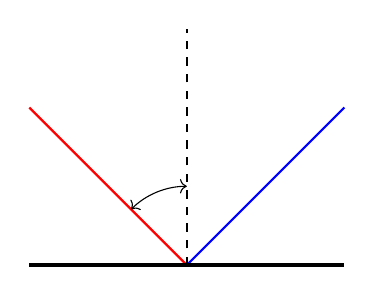
\begin{tikzpicture}
        \draw[  red, thick] (0, 0) -- (2,-2);
        \draw[ blue, thick] (2,-2) -- (4, 0);
        \draw[black, very thick] (0,-2) -- (4,-2);

        \draw[black, thick, dashed] (2,-2) -- (2, 1);

        \draw[<->] (2,-1) arc (90:135:1);
    \end{tikzpicture}
    \end{center}
\end{figure}

Since reflection does not change the wavelength/frequency of light, the wavelength($\lambda$)
and frequency($f$) remains same:

\begin{align}
    \lambda &= 5000\AA\\
    f &= \frac{c}{\lambda}\\
    &= 6 \cdot 10^{15} {Hz}
\end{align}

The reflected ray is normal to incident ray for angle of incidence $ = 45\deg$.

\end{document}
